\documentclass[../main.tex]{subfile}
\begin{document}
\section{Shader computation and foliage}
In this section we are going to see how storing the three dimensional force field in a 2D texture can be used to move the verticies of the foliage.
For this purpose we are going to use render targets and more specifically blend between two render targest (called here buffers) to achieve an
optimised dynamic wind evolution on the foliage.\\

The way to pass datas to a shader is to use textures. We are going to encode the 3D vector representing direction of the wind in each pixel. The coordinate 
of the pixel can then be mapped on the world position. By doing so we can play with the UV of the texture to sample the wind force at the location where the pixel 
(of the 3D scene on the viewport) is located. This system is very good scalable so if you want to lower of higher the resolution of the wind, you can improve the resolution
of the render target. A resolution of $64\times64$ pixel was found to be a pretty good value for a $200k\times200k$ unit sqaured map.\\

\textbf{Note:} (for mathematians or phisicians) The following uses the force field as a $\bm{k}$ ``momentum'' field to displace the shader.

\subsection{Capturing the 2D texture}
The first step is to capture the 3D texture. Trained eyes will have noticed that a texture is 2D and not 3D. This means we can only store, per texture, a \textit{slice} of the world 
to make the tree shake. A realistic aproach would be to have mutliple textures that we can choose according on the $z$ value. However this is going to cost
us a lot of memory so we are going to use a trick.\\

If we think about it, the terrain is just a texture elevated along the $z$ axis, in other words if we look at it from the top, it looks flat. This means, instead of 
storing multiple slices, we could make some traces from the sky to the ground to store the $z$ location of the terrain, where we expect the trees to be.\\

\paragraph{Getting the plane $xy$-coordinates} $~$ To find the right transformation between the world coordinate (XY) and the texture coordinate (UV) we can start with a scheme.
Here we supperpose the UV and the XY origin.\\

\begin{center}
    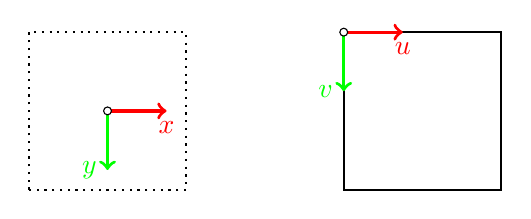
\begin{tikzpicture}
        \draw[draw=black,  thick] (3,-1) rectangle ++(2,2);
        \draw[->, color = red, very thick] (3,1) -- ++(.75,0) node[anchor=north] {$u$};
        \draw[->, color = green, very thick] (3,1) -- ++(0,-.75) node[anchor=east] {$v$};
        \draw[draw=black,  thick, dotted] (-1,-1) rectangle ++(2,2);
        \draw[->, color = red, very thick] (0,0) -- ++(.75,0) node[anchor=north] {$x$};
        \draw[->, color = green, very thick] (0,0) -- ++(0,-.75) node[anchor=east] {$y$};
        \filldraw[color=black, fill = white , thin] (0,0) circle (0.05);
        \filldraw[color=black, fill = white , thin] (3,1) circle (0.05);
    \end{tikzpicture}
\end{center}
\begin{center}
    \begin{tikzpicture}
        \draw[draw=black,thick] (0,-1.5) rectangle ++(1.5,1.5);
        \draw[draw=black,thick, dotted] (-2,-2) rectangle ++(4,4);
        \node[rectangle, draw=none, minimum size=1pt] at (0.75, -1.7) {\(n\)};
        \draw[->, color = red, very thick] (0,0) -- ++(1,0) node[anchor=north] {$x,u$};
        \draw[->, color = green, very thick] (0,0) -- ++(0,-1) node[anchor=east] {$y,v$};
        \filldraw[color=black, fill = white , thin] (0,0) circle (0.05);
        \node[rectangle, draw=none, minimum size=1pt] at (0, -2.2) {\(m\)};
    \end{tikzpicture}
\end{center}
An important information has to be highlighted, UE works in a left handed coordinate system. This means that the $v$ axis is pointing down. This differs from the conventions 
in mathematics/physics where the $y$ axis is pointing up.\\
So the first step is to scale the texture to fill the world size and then replace the center of the UV to the top left corner of the XY terrain. We can take a coordinate $\bm{r}(x,y)$
on the landscape and write a transformation to get the UV coordinate $\bm{k}(u,v)$.
\[
    \bm{r}(x,y) = \bm{k}(u,v) \frac{m}{n} - \frac{m}{2}\begin{pmatrix}1\\1\end{pmatrix}
\]
In the same way the transformation from the world coordinate to the UV are:
\[
    \bm{k}(u,v) = \left(\bm{r}(x,y) + \frac{m}{2}\begin{pmatrix}1\\1\end{pmatrix}\right) \frac{n}{m}
\]
which is the inverse process. We first move the world coordinate so that the upper left corner lays on the origin of the UV and then we scale it down.\\

This transformation can be found in the shader material function \texttt{MF\_WindDeform}. The convention is to have $\bm{k}(u,v)$ using $u,v$ betweem 0 and 1. 
In such circumstances we have $n=1$.
\begin{figure}[H]
    \centering
    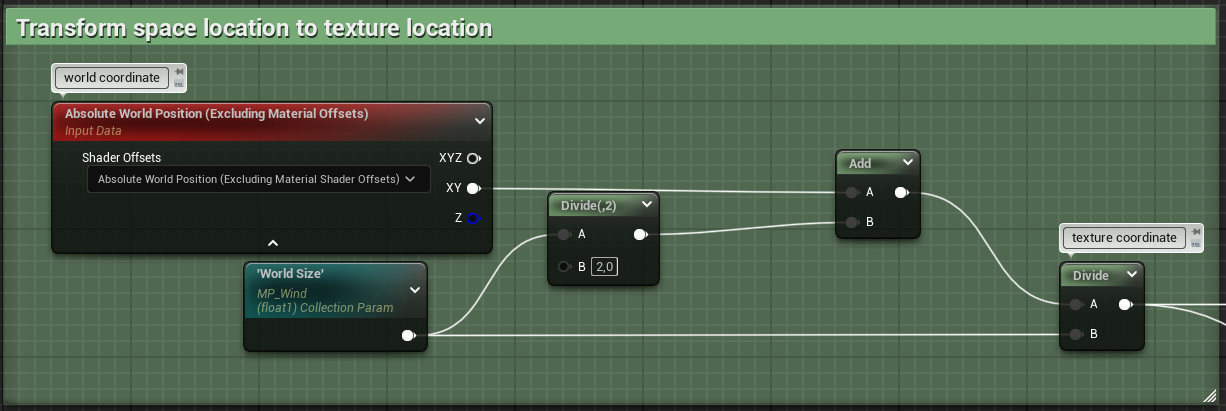
\includegraphics[width=1\textwidth]{Ressources/RealSpaceToUV.png}
    \caption{The transformation from the world coordinate to the UV coordinate. The \texttt{World Size} scalar parameter is the world side length $m$.
    In the default UE5 project this is $200k$ units. You should set it to the size of your world. If too small you may see the wind patern repeat itself
    and having some discontinuities on the edges. On the other hand, if too big, you will project only a part of the world on the texture.}
\end{figure}

We can then find to a map location the corresponding pixel in the texture to write the force at. 
\begin{figure}[H]
    \centering
    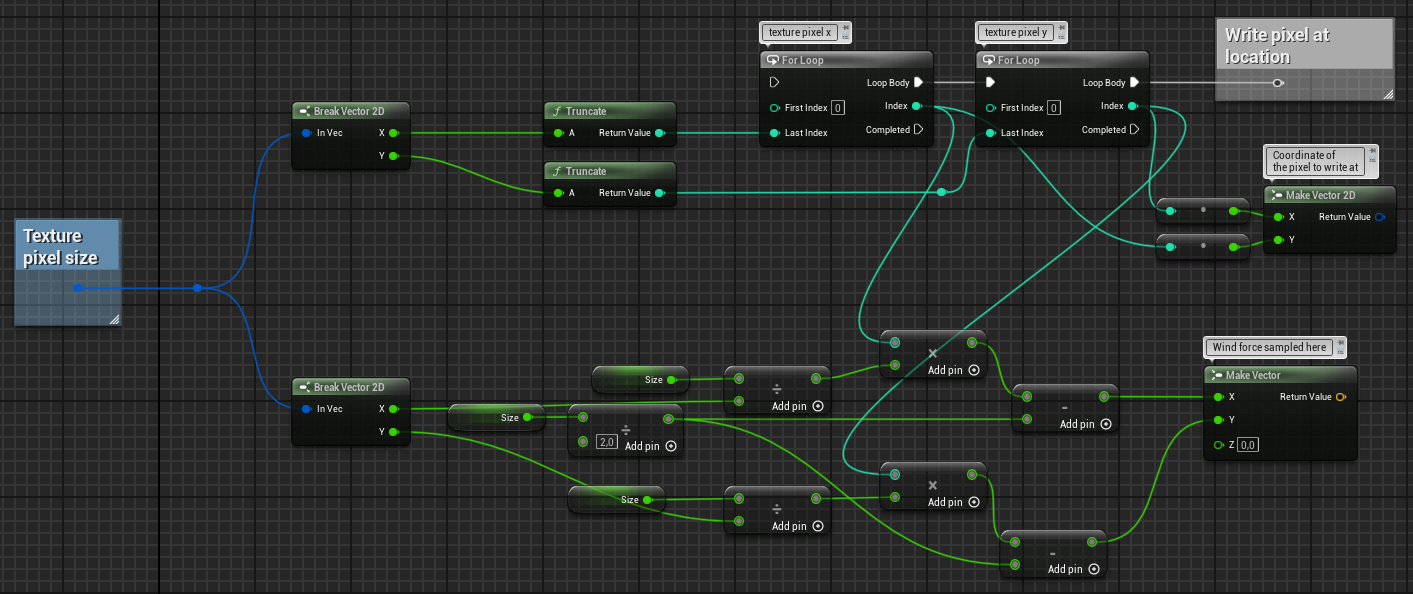
\includegraphics[width=1\textwidth]{Ressources/WritePixelAtLoca.png}
    \caption{How we determine the pixel location from the world position. The texture beeing $64\times64$ pixels, a U of 1 corresponds to 64 pixels.}                                                                       
\end{figure}

\paragraph{Getting the $z$-coordinate} $~$ The next step is to get the elevaion $z$-coordinate. This is done by casting a ray from the sky to the ground. Since the 
terrain is flat and stays roughly the same during the runtime, this only need to be made one at the beggining og the game. For the $x$ and $y$ coordinate we can base ourselves on the texture size as just discussed.
The trace should start a bit above the heighest point of the map and end a bit below the lowest point. Then we can store the $z$ value in an array to find
the force later at this heigh.\\

However there is no possbility to write matrcies in UE5 where the enrty index would be the x and y coordinate and the value the $z$ coordinate. However
we can imagine puting this matrix row by row in a array. This means if the world in $10\times10$, the first 10 values of the array describe the z coordinate from 
(1,1) to (1,10), the next 10 values from (2,1) to (2,10) and so on. The general formula is then:
\[
    \text{index} =(y-1)\cdot x
\]
this is achieved in \texttt{BP\_WindManager::ComputeHeight}. Knowing in advanced that the array should be $N_x \cdot N_y$ items long, 
we can already preallocate the entries to save some time. We can use the same forula to get the $z$ value out of the array while writing the wind.\\

\subsection{Writing the wind}
Now that we have the actual position, we can use our force field to sample the strength and direction of the wind at that location. The main problem is now how we
are going to encode this in a texture. Well, the strength is represented by three components, the $x$, $y$ and $z$ component of the force. We can then use the red, green and blue
channel of the texture to store this information. However if the wind points in $(-1,-1,-1)$ or has any negative values, we are going to have a problem. In fact the 
way texture are encoded restricts us in the use of negative values. All the values has to be maped between 0 and 1. There is fortunately a methode to store negative values, which is also used in normal maps. An
exemple involving a sinusoidal wave can be helpful.\\
\begin{figure}[H]
    \centering
\begin{tikzpicture}
    \begin{axis}[
        axis lines=middle,
        width=6cm,   % Adjust the width
        height=4cm,  % Adjust the height
        xlabel={$x$},
        xtick=\empty,
        ylabel={$y$},
        ymin=-2.2, ymax=2.2,
        samples=100,
        domain=-8:8
    ]
        % Plot a cosine function
    \addplot[smooth, variable=\x, TamRosa, thick] ({\x}, {cos(deg(\x))});
    \end{axis}
    \node[rectangle, draw=none, minimum size=1pt] at (2, -.7) {\(\cos(x)\)};
\end{tikzpicture}
\begin{tikzpicture}
    \begin{axis}[
        axis lines=middle,
        width=6cm,   % Adjust the width
        height=4cm,  % Adjust the height
        xlabel={$x$},
        xtick=\empty,
        ymin=-2.2, ymax=2.2,
        ylabel={$y$},
        samples=100,
        domain=-8:8
    ]
        % Plot a cosine function
        \addplot[smooth, variable=\x, TamYellow, thick] ({\x}, {cos(deg(\x))+1});
    \end{axis}
    \node[rectangle, draw=none, minimum size=1pt] at (2, -.7) {\(\cos(x)+1\)};

\end{tikzpicture}
\begin{tikzpicture}
    \begin{axis}[
        axis lines=middle,
        width=6cm,   % Adjust the width
        height=4cm,  % Adjust the height
        xlabel={$x$},
        xtick=\empty,
        ymin=-2.2, ymax=2.2,
        ylabel={$y$},
        samples=100,
        domain=-8:8
    ]
        % Plot a cosine function
        \addplot[smooth, variable=\x, TamDarkBlue2, thick] ({\x}, {(cos(deg(\x))+1)/2});
        
    \end{axis}
    \node[rectangle, draw=none, minimum size=1pt] at (2, -.7) {\((\cos(x)+1)/2\)};
\end{tikzpicture}
\end{figure}
By doing so, we have stored the same information (the curve shape) in the zero to one range. Whene decoding we value we should do the opposite operation otherwise our wind will only
show in the poisitve direction with a maximal strength of 1. Asuming that the maximal value of a function $f_{\text{real}}$ should be $f_{max}$, we have
\[
    f_{\text{encoded}} = \left(\frac{f_{\text{real}}}{f_{\text{max}}} + 1\right)\frac{1}{2}.
\]
\begin{figure}[H]
    \centering
    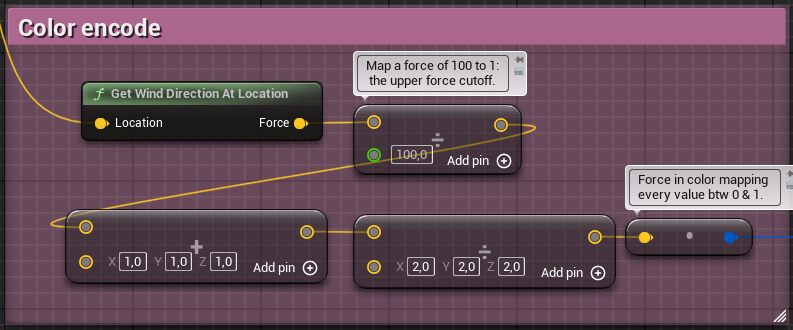
\includegraphics[width=.7\textwidth]{Ressources/ColorEncode.png}
    \caption{We treat our signal as the force and map every component between 0 and 1 according to the upper scheme.}
\end{figure}

The deocde when sampling the texture is then simply $f_{\text{real}} = 2f_{\text{encoded}}\cdot f_{\text{max}} -1$. This is done in \texttt{MF\_WindDeform}.\\

\paragraph{Achieving dynamic shader wind} $~$ Until now, when we recompute the wind for the shader and therefore modify the texture, we observe a 
sudden change in the wind patern if the force field has changed. This is due to the fact that we are directly writing the new wind in the texture.
A first way to solve this would be to recompute the texture every tick. This is however a demanding operation. The BP script is executed on the CPU.
Writing the texture takes however place on the GPU. Now a second important information. The code can run on a thread. It's basically an instruction line. Like you 
would be in a queue. Whene an instruction does something, this blocs the whole thread (queue). Writing the texture takes some time because the information travel
from the CPU to the GPU and then back to tell the GPU is finished. In this sense writing a texture a blocking operation.\\

Now the sad part about it is that if this queue happens to be the ``game thread'', the game will freeze until the texture is written. This causes periodical anoying freezes.
The first solution would be to write the texture every 10s for exemple, store it and interpolating between the two textures stored in $A$ and $B$ to acheive a dynamic transition between the two states.

\begin{center}
    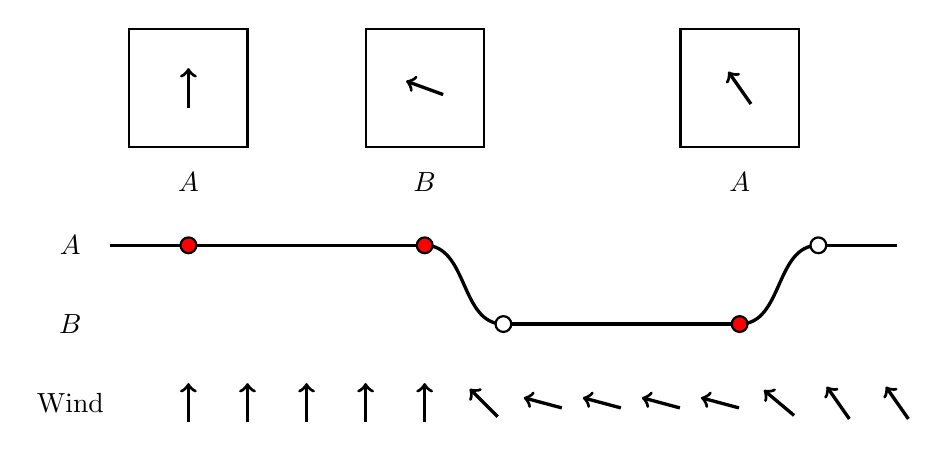
\begin{tikzpicture}
        \coordinate (A) at (0,0);
        \draw[draw=black,thick] (A)++(-0.75, -0.75) rectangle ++(1.5,1.5);
        \draw[->, very thick] (A)++(0,-0.25) -- ++(0,0.5) ;
        \coordinate (B) at (3,0);
        \draw[draw=black,thick] (B)++(-0.75, -0.75) rectangle ++(1.5,1.5);
        \draw[->, very thick,rotate around={70:(B)}] (B)++(0,-0.25) -- ++(0,0.5) ;
        \coordinate (C) at (7,0);
        \draw[draw=black,thick] (C)++(-0.75, -0.75) rectangle ++(1.5,1.5);
        \draw[->, very thick,rotate around={35:(C)}] (C)++(0,-0.25) -- ++(0,0.5) ;

        \node[rectangle, draw=none, minimum size=1pt] at (0, -1.2) {\(A\)};
        \node[rectangle, draw=none, minimum size=1pt] at (3, -1.2) {\(B\)};
        \node[rectangle, draw=none, minimum size=1pt] at (7, -1.2) {\(A\)};

        \draw[-, very thick] (-1,-2) -- (3,-2);
        \draw[-, very thick] (3,-2) to[out=0, in=180] (4,-3);
        \draw[-, very thick] (4,-3) -- (7,-3);
        \draw[-, very thick] (7,-3) to[out=0, in=180] (8,-2);
        \draw[-, very thick] (8,-2) -- (9,-2);
        \filldraw[color=black, fill = red , thick] (0,-2) circle (0.1);
        \filldraw[color=black, fill = red , thick] (3,-2) circle (0.1);
        \filldraw[color=black, fill = white , thick] (4,-3) circle (0.1);
        \filldraw[color=black, fill = red , thick] (7,-3) circle (0.1);
        \filldraw[color=black, fill = white , thick] (8,-2) circle (0.1);
        \node[rectangle, draw=none, minimum size=1pt] at (-1.5, -2) {\(A\)};
        \node[rectangle, draw=none, minimum size=1pt] at (-1.5, -3) {\(B\)};
        \node[rectangle, draw=none, minimum size=1pt] at (-1.5, -4) {Wind};

            % Add arrows below the curve
        \foreach \x/\angle in {0/0, 0.75/0, 1.5/0, 2.25/0, 3/0, 3.75/45, 4.5/75, 5.25/75, 6/75, 6.75/75, 7.5/50, 8.25/35, 9/35 } {
            \draw[->, very thick, rotate around={\angle:(\x,-4)}] (\x,-4.25) -- ++(0,0.5);
        }
    \end{tikzpicture}
\end{center}
In this timeline, the red dots correspond to the storing of the texture in the cooresponding buffer. When a new buffer is written, the wind is interpolated between
the current buffer and the newly written buffer. Resulting in a continuous wind evolution, even if the wind is only captured three times.
This is achieved in \texttt{BP\_WindManager::CacheNewWind} and the actual update is done in the tick.\\
The function we use there to interpolate is an hyperbolic tangent. This looks very similar to a besier curve. We have to shift it have the slopes bewteen 0 and 1 
because it's nicer to work with. Additionaly the whole slope should be mapped using an $x$ between 0 and 1, so we have to increase the exponent to make this slope stronger.
In the limit of $x$ going to infinity, the function is a step at 0.5. Going back means simply starting from zero and inverting the curve, what is done with the $(1-x)$ in the 
select node.\\

\begin{figure}[H]
    \centering
    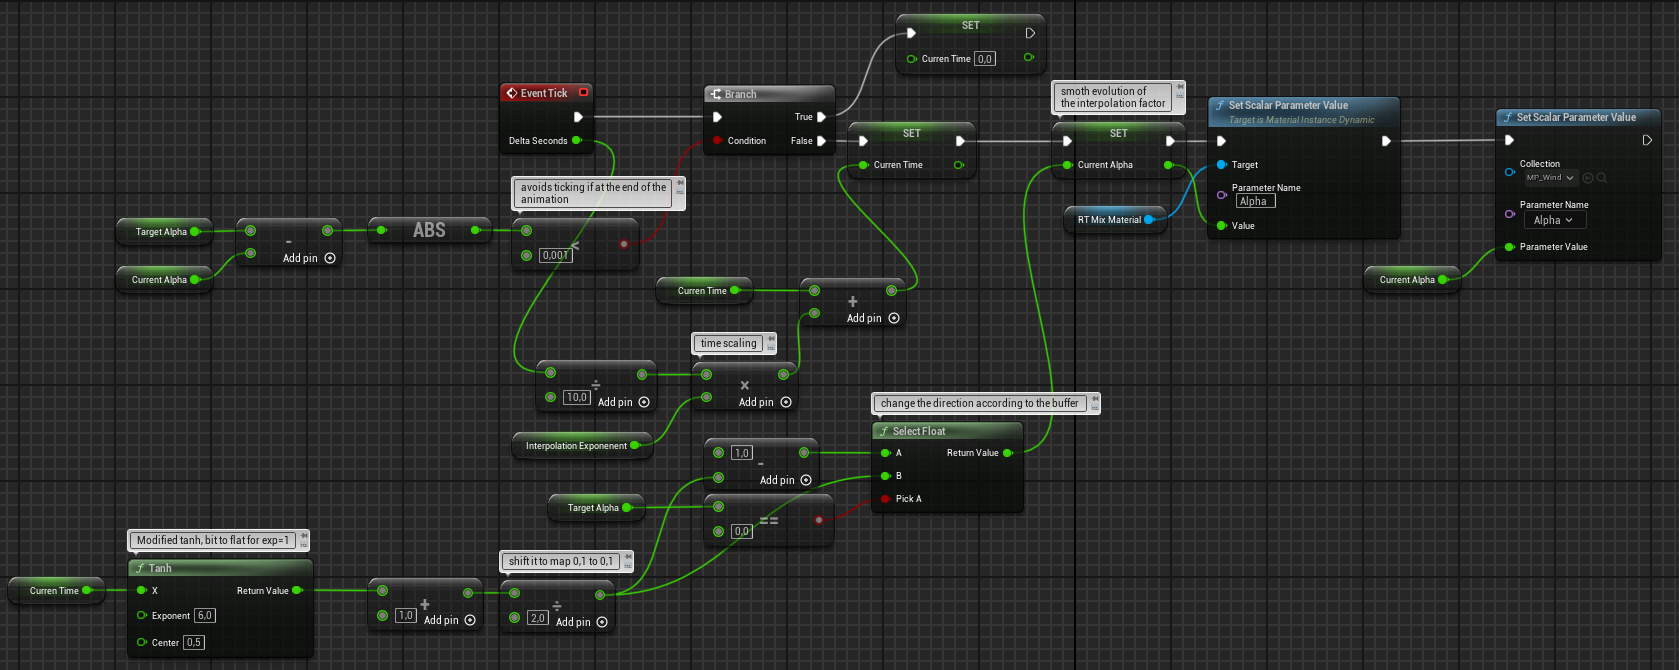
\includegraphics[width=1\textwidth]{Ressources/AlphaInterpolation.png}
    \caption{The interpolation function used to blend between the two textures. The actual shader interpolation is just a lerp between the two textures and is
    found in \texttt{MF\_WindDeform}.}   
\end{figure}

\subsection{Applying the wind on the foliage}
The breakdown of the shader itself quit simple. First we need to displace the verticies in the direction stored at by the texture. Second we can progagate a wave trough the foliage.
For the later one, you might familiar with the use of a normal map combined to a WorldAlignedTextures used in grass shaders to achieve a wavy effect. Well, we are going to use
something more simple but wich work very good as well and follows the lines.\\

This is directly inspiered by the theorie of the plane wave propagation in physics. Asuming that the wave propagates itself along the $\bm{k}$ vector, we have 
for the amplitude of the wave at a given point $\bm{r}$ and time $t$ \url{https://en.wikipedia.org/wiki/Sinusoidal_plane_wave}:
\[
    A(\bm{r},t) = A_0 \sin(\bm{k}\cdot \bm{r} - \omega t + \varphi)
\]
$\bm{k}\cdot \bm{r}$ describes a scar product and is a scalar gien as $k_xr_x + k_yr_y + k_zr_z$. Another description is the following:
\[
    \bm{k}\cdot \bm{r} = |\bm{k}||\bm{r}|\cos(\theta)
\]
where $\theta$ is the angle between the two vectors. If $\theta$ is $90$ or $-90$ degrees, the cosine is null and this term dosn't contribute to the phase of the wave. This means,
if this angle is observed bewteen the velocity and the location we get 0. On the other hand if the velocity is aligned with the vector position, the phase contribution is maximal
and the tree  is going to be a bit in advance than the other locations.\\

The $\omega t$ term is the time evolution of the wave, which allows the propagation of the wave. The $\varphi$ term is an additional phase for the wave. This can be used to add some
delay in a tree if it's bigger for exemple.\\

Now we can multiply this oscillation with the wind displacment to acheive a ``real'' wave propagation. However the sine gives values between -1 and 1. This means that the tree is going to
move back an forth. This is not exactly what we want. The tree can become straigth again but it doesn't tilt in the opposite direction of the wind. This means we want to exclude
the negative values but still want to keep the complete oscillation. This can be done with the similar methode we saw earlier to encode the texture with $(\sin(x)+1)/2$.\\
\begin{figure}[H]
    \centering
    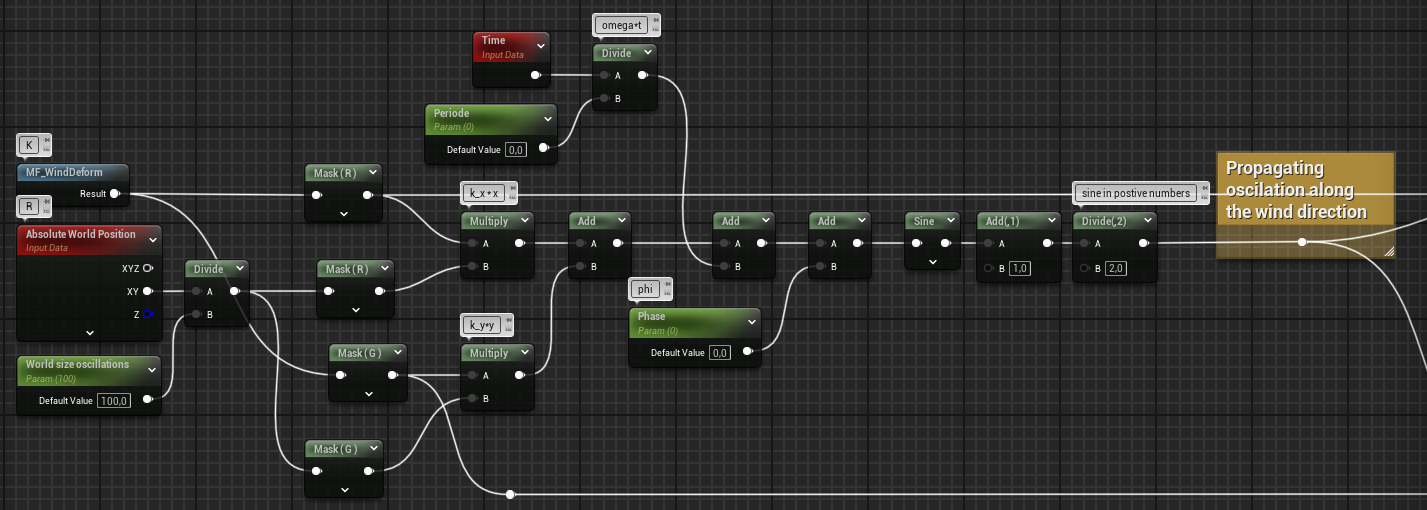
\includegraphics[width=1\textwidth]{Ressources/PropagatingOscillation.png}
    \caption{The propagating oscillation as an amplitude dependent of the location. The sine wave is then shifted to have only positive values.}
\end{figure}

However now we get an oscillation between 0 and 1 but we don't have any vector to displace along. Now we can simply multiply the oscillation with the wind vector on each 
component $x$ and $y$. The $z$ component, we want the tip of the tree to move a bit down. We combine bothe the $x$ and $y$ oscillation, scale it down and use this for the $z$ component.\\
\begin{figure}[H]
    \centering
    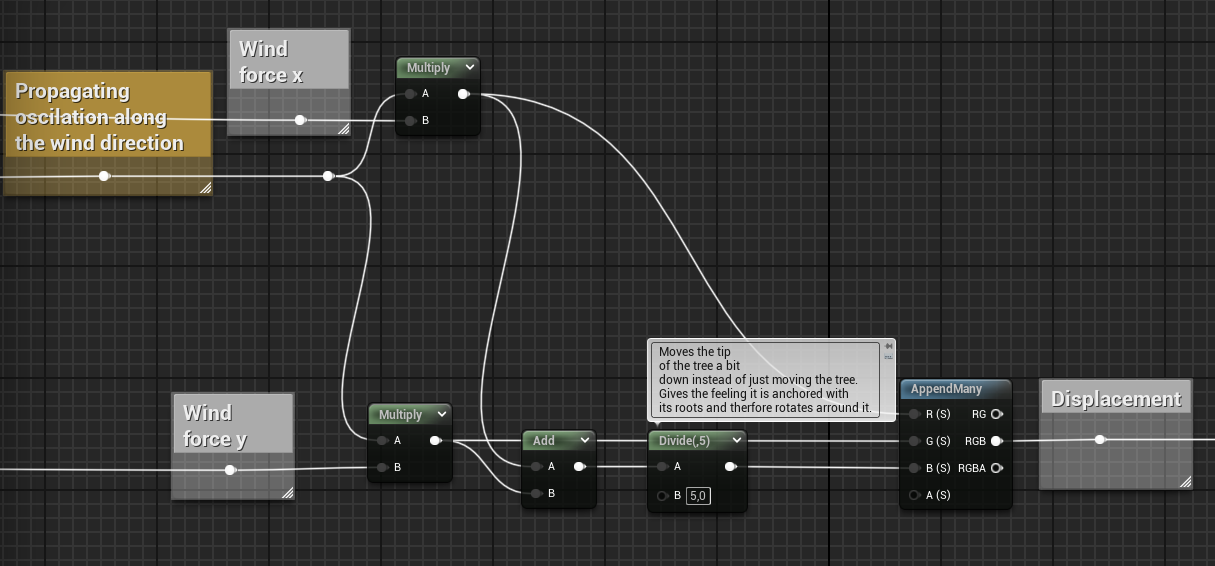
\includegraphics[width=1\textwidth]{Ressources/OscillationCombineVectors.png}
    \caption{The final displacement of the tree. The oscillation is multiplied with the wind vector to get the final displacement.}
\end{figure}

However now we get a uniform displacement for the complete tree. The tree just slides and come back. We want its top to move and its bottom to be fixed. In other words 
there is a gradient in the displacement from fixed verticies on the roots to a fully moving top of the tree. To do this we can use the UV of the trees.

We can then simply use the $z$ position of the verticies in the tree space and map it between 0 and 1. 1 beeing the point at which the tree receive the full displacement of the wind.
You can adjust this using the parameter \texttt{Folliage Top} in the material. These should be unreal units.\\
\begin{figure}[H]
    \centering
    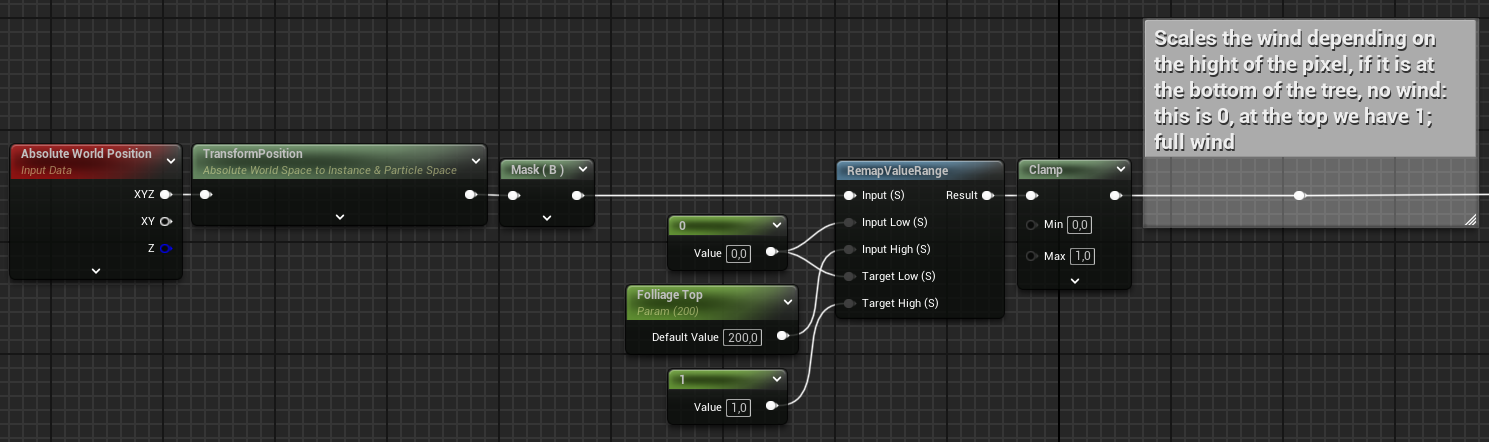
\includegraphics[width=1\textwidth]{Ressources/WindGradient.png}
    \caption{The gradient displacement of the tree. The top of the tree is fully displaced by the wind while the bottom is fixed. This scalar just multiplies the displacement 
    we descriped.}
\end{figure}
Finely a strengh can be ajusted if a folliage is bigger it will obviouly not move very far.

\subsection{Complexer movement}
You may have noticed that the wind is not only a simple oscillation and it looks very peacfull like the bottom of the sea. The real wind has some bursts and more chill
movments sometimes. We need a complexer signal with tiny oscillations and strong ones overlapping.

\begin{figure}[H]
    \centering
\begin{tikzpicture}
    \begin{axis}[
        axis lines=middle,
        width=6cm,   % Adjust the width
        height=4cm,  % Adjust the height
        xlabel={$x$},
        xtick=\empty,
        ylabel={$y$},
        ymin=-2.2, ymax=2.2,
        samples=100,
        domain=-8:8
    ]
        % Plot a cosine function
    \addplot[smooth, variable=\x, TamDarkBlue2,thick] ({\x}, {sin(deg(\x))});
    \end{axis}
    \node[rectangle, draw=none, minimum size=1pt] at (2, -.7) {\(\sin(x)\)};
\end{tikzpicture}
\hspace{1cm}
\begin{tikzpicture}
    \begin{axis}[
        axis lines=middle,
        width=6cm,   % Adjust the width
        height=4cm,  % Adjust the height
        xlabel={$x$},
        xtick=\empty,
        ymin=-2.2, ymax=2.2,
        ylabel={$y$},
        samples=100,
        domain=-8:8
    ]
        % Plot a cosine function
        \addplot[smooth, variable=\x, TamLightGreen, thick] ({\x}, {sign(sin(deg(\x)))});
    \end{axis}
    \node[rectangle, draw=none, minimum size=1pt] at (2, -.7) {\(\text{sign}(\sin(x))\)};
\end{tikzpicture}
\vspace{1cm}\\
\begin{tikzpicture}
    \begin{axis}[
        axis lines=middle,
        width=6cm,   % Adjust the width
        height=4cm,  % Adjust the height
        xlabel={$x$},
        xtick=\empty,
        ymin=-1.2, ymax=1.2,
        ylabel={$y$},
        samples=100,
        domain=-8:8
    ]
        % Plot a cosine function
        \addplot[smooth, variable=\x, TamLightGY,thick] ({\x}, {max(sign(sin(deg(\x))), 0) + 0.08*cos(10*deg(\x))});
    \end{axis}
    \node[rectangle, draw=none, minimum size=1pt] at (2, -.7) {\(\text{Max}(\text{sign}(\sin(x)), 0)+ 0.05\cdot\cos(10\cdot x)\)};
\end{tikzpicture}
\begin{tikzpicture}
    \begin{axis}[
        axis lines=middle,
        width=6cm,   % Adjust the width
        height=4cm,  % Adjust the height
        xlabel={$x$},
        xtick=\empty,
        ymin=-1.2, ymax=1.2,
        ylabel={$y$},
        samples=100,
        domain=-8:8
    ]
        % Plot a cosine function
        \addplot[smooth, variable=\x, TamYellow,thick] ({\x}, {max(sign(sin(deg(\x))), 0)*sin(deg(\x))*sin(deg(\x)) + 0.08*cos(10*deg(\x))});
        
    \end{axis}
    \node[rectangle, draw=none, minimum size=1pt] at (2, -.7) {\(\text{Max}(\text{sign}(\sin(x)), 0)\cdot\sin(x)^2 + 0.05\cdot\cos(10\cdot x)\)};
\end{tikzpicture}
\end{figure}
After doing this construction, we see that we obtain some moments with strong wind and some where just the tiny, chill oscillations are present.\\
To activate this more complexe wave paterns you can check the \texttt{Complex Wind} in the material. This will be done in the cost of 18 additional instructions.\\

The next level will be to shake the leaves of the tree, beacause for now the tree moves as a mass, treeting the leaves in the same way as the trunc. To do so
we can inspire us from the tiny oscillations just presented. Morover we could use the relative heigth of the leaf to make the small shake propagate along the height of the tree.
This means we would just have some delay along the heigth. 
Recalling that the phase can add some delay, we can directly use the heigth information as a phase. Depeneding on the wind strength we can make
this oscillations go faster by multipling the time with the speed making for a twice as strong wind, some twice as rapid oscillations. To apply this leaf
movements, check the \texttt{Is a leaf} parameter\\
\begin{figure}[H]
    \centering
    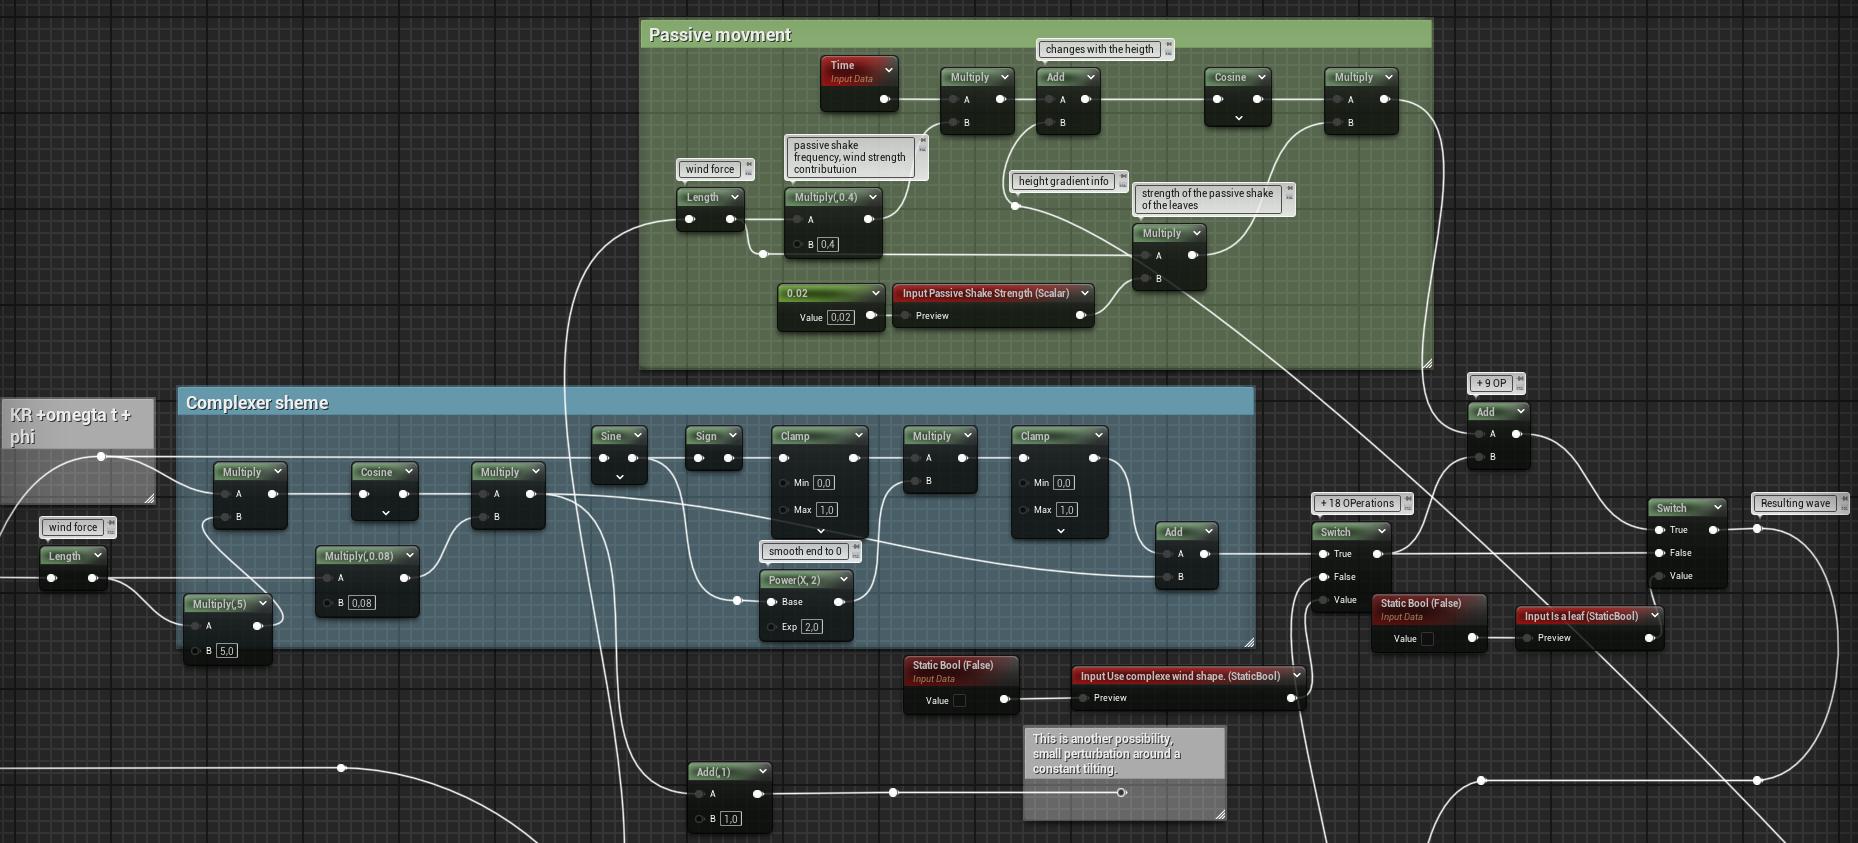
\includegraphics[width=1\textwidth]{Ressources/ComplexeWave.png}
    \caption{The possbility to activate the passive leaf shake and the global complexer wind patern involving bursts and chill oscillations.}
\end{figure}
